\section{Formazione delle galassie}\label{sec:formazione-delle-galassie}
\subsection{Galassie interagenti}
Capita spesso che le galassie non siano isolate ma si trovano in interazione con delle altre; in particolar modo spesso si tratta di eventi di collisione o di "cannibalismo" (una galassia che ne assorbe un'altra) ed ovviamente questi eventi modificano la morfologia galattica. Il merge di galassie sembra essere quindi all’origine della diversa composizione morfologica delle galassie e spesso è un catalizzatore di formazione stellare; infatti quando si ha una “collisione” si ha una compressione del gas, che quindi, aumenta la densità e ciò favorisce la formazione stellare.

\subsection{Processi di formazione}
Capire come si formano le galassie è uno dei problemi più complicati, perché in questo processo intervengono tantissimi fenomeni fisici. Un elenco non esaustivo dei processi coinvolti sono: effetti gravitazionali, raffreddamento, riscaldamento e turbolenza di gas, formazione stellare, feedback provenienti dal buco nero centrale, problemi di frammentazione o instabilità del disco, fusione fra galassie, evoluzione chimica, campi magnetici, ...

L'idea di base della formazione delle galassie è che prima si formi un alone di materia oscura; dopodiché la materia barionica collassa all'interno di questo alone e si forma la galassia. Per quanto riguarda gli aloni di materia oscura, bisogna considerare solamente le forze di gravità: è sufficiente fare dei modelli a N corpi in cui si considera solamente la mutua attrazione gravitazionale, quindi questa parte presenta come unica difficoltà il dispendio computazionale. Per ciò che riguarda la componente barionica invece lo studio è molto più difficile, essendo essa soggetta a molte forze. Sono presenti diversi approcci:
\begin{itemize}
    \item Simulazioni idrodinamiche: le particelle sono particelle di gas, quindi oltre alla gravità calcoliamo i processi termodinamici relativi a un gas. Si tratta di un approccio molto più preciso, ma questi calcoli sono molto dispendiosi computazionalmente.
    \item Modelli semi-analitici: approssimiamo e semplifichiamo la situazione dal punto di vista di calcolo nelle simulazioni a N corpi. Le approssimazioni sono grossolane ma è possibile cambiare i parametri del modello senza dover aspettare ogni volta tanto tempo per far riandare la simulazione, quindi è possibile ripetere le simulazioni più e più volte (molto versatili).
    \item Modelli individuali per aspetti specifici: si costruiscono modelli che prendano in considerazione solo un processo, come ad esempio modelli di evoluzione chimica, modelli dinamici, \dots 
\end{itemize}

Ad oggi non esiste un modello di formazione delle galassie che sia soddisfacente; infatti ogni modello presente è in grado di spiegare alcuni aspetti ma fallisce nello spiegare altre proprietà. Vediamo quindi due quadri, uno più vecchio-stile e uno più moderno che tentano di spiegare i processi di formazione delle galassie.

\subsubsection{Visione vecchio-stile sulla formazione delle galassie}
La visione vecchio-stile del problema da una buona idea della fisica della formazione delle galassie. Partiamo da un alone di materia oscura con, all’interno, una nube di gas barionico. Possono succedere due cose principali:
\begin{itemize}
    \item  Collasso dissipativo: si parla di collasso dissipativo quando c’è perdita di energia (= dissipazione) nel collasso della nube di materia oscura. Immaginando che ci sia una rotazione iniziale della nube si ha che il momento angolare si conserva e di conseguenza il piano di rotazione; quindi il gas non collassa sfericamente ma si posiziona lungo un disco rotante perpendicolare al momento angolare. In questo disco rotante fatto di gas si formano le stelle: in questa maniera si forma una galassia a disco.
    \item Collasso non dissipativo: c’è un collasso non dissipativo quando non si ha perdita di energia del gas all'interno della nube. L’idea è che il tasso di formazione stellare sia maggiore del tasso di dissipazione del gas (quindi che il tempo scala della formazione stellare sia minore del tempo scala di dissipazione del gas): quindi si ha una sfera di gas e quella che sta collassando è la distribuzione di stelle. Non si ha dunque dissipazione (non si ha un gas, ma stelle, ovvero masse puntiformi, quindi assistiamo ad un collasso gravitazionale) e rimane la simmetria sferica della distribuzione di particelle, che diminuisce in volume; al contrario del caso precedente quindi non abbiamo uno schiacciamento con conseguente creazione di una galassia a disco. Come si raggiunge l’equilibrio? L’idea del 1967 di Lyndel-Bell è quella del rilassamento  violento: durante il collasso varia il potenziale gravitazionale nel tempo quindi c’è una ridistribuzione di energie nelle particelle. È come se ci fossero delle collisioni tra le stelle, ma non accade realmente. Questa redistribuzione di energie permette di raggiungere l’equilibrio: in questa maniera si forma una galassia sferoidale.
\end{itemize}

\begin{figure}
    \centering
    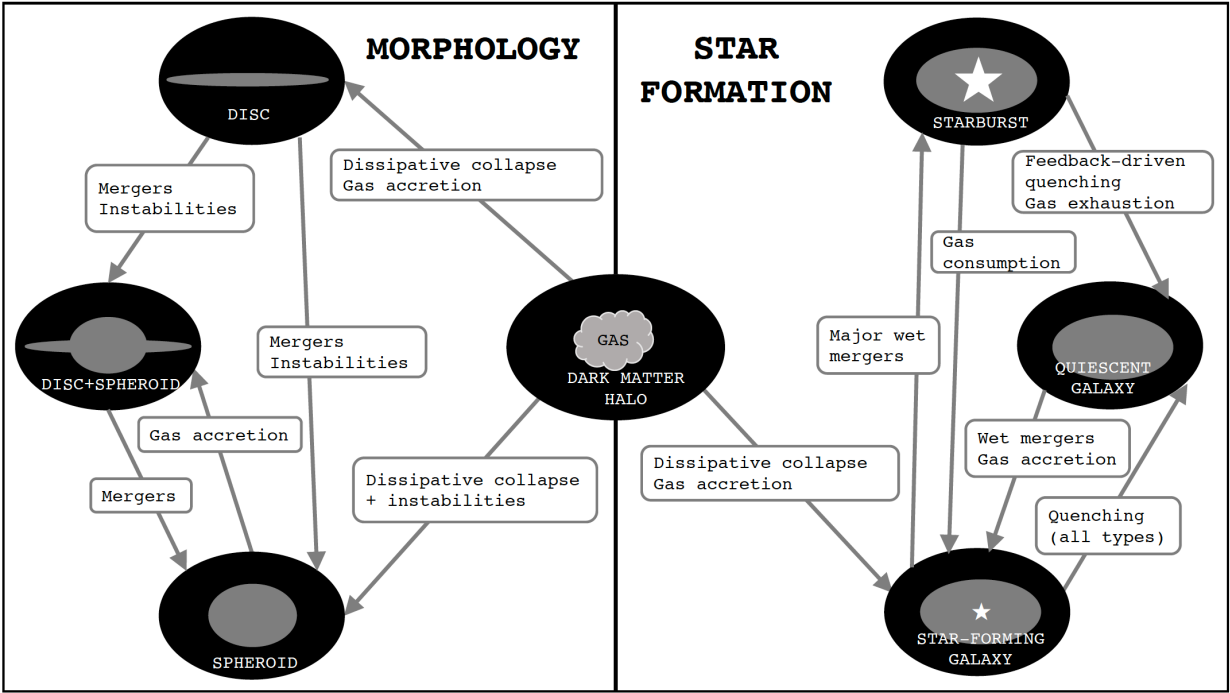
\includegraphics[width = \textwidth]{immagini/formazione-delle-galassie-visione-moderna.png}
    \caption{Riassunto della visione moderna del processo di formazione delle galassie (visione ancora incompleta).}
    \label{fig:formazione-delle-galassie-visione-moderna}
\end{figure}

\subsubsection{Visione moderna sulla formazione delle galassie}
Una visione più moderna della situazione, anche se non completa, è la seguente (riassunta in figura~\ref{fig:formazione-delle-galassie-visione-moderna}). Partiamo nuovamente da un alone di materia oscura con gas all’interno; questa visione ci permette di dare una spiegazione sia alla morfologia sia alla presenza delle stelle e ai vari tipi di produzione stellare nelle galassie.

\begin{itemize}
    \item \emph{MORFOLOGIA}: per quanto riguarda la morfologia, dall'alone di materia oscura abbiamo un collasso dissipativo del gas al suo interno. Se non sono presenti instabilità allora si forma una galassia a disco (quindi avviene lo schiacciamento sul piano di rotazione), mentre se sono presenti instabilità si crea una galassia sferoidale, perché le instabilità frantumano il disco. A questo punto il merge fra varie galassie a disco può dar luogo o a galassie sferoidali o a galassie del tipo a disco con uno sfeoride (bulge) centrale. A loro volta queste galassie a disco con bulge possono fare dei merger che danno luogo a uno sferoide.
    \item \emph{FORMAZIONE STELLARE}: per riprodurre non la morfologia ma le proprietà di formazione stellare delle galassie, consideriamo uno scenario diverso. Partiamo da un gas di materia oscura che collassa con dissipazione e in seguito c’è accrescimento di gas. Si forma una galassia che sta formando stelle (questo perchè aumenta la densità quindi la porbabilità di dar luogo a stelle). Però il problema è che non tutte le galassie che osserviamo stanno formando stelle (ad esempio le galassie ellittiche sono quiescenti), mentre d’altra parte le galassie star-burst hanno una intensissima formazione stellare. Come possono formarsi questi due tipi di galassie? Si hanno varie possibilità:
    \begin{itemize}
        \item Per quanto riguarda le galassie ellittiche quiescenti possono entrare in gioco dei processi di spegnimento si oppongono alla formazione stellare e danno luogo a queste galassie.
        \item Per quanto riguarda le galassie starbust, se abbiamo un merge fra due galassie di massa confrontabile e che contengono entrambe gas (major wet merger\footnote{
        MAJOR MERGER: merger fra galassie di massa comparabile. \\
        WET MERGER: merger fra galassie ricche di gas.
        }) abbiamo condizioni molto favorevoli alla produzione stellare e quindi possiamo creare una galassia starbust.
    \end{itemize}
\end{itemize}